\documentclass{article}
 
%Russian-specific packages
%--------------------------------------
\usepackage[T2A]{fontenc}
\usepackage[utf8]{inputenc}
\usepackage[russian,english]{babel}
\usepackage{graphicx} 
\usepackage{amsmath}
\usepackage{amssymb}
\usepackage{url} 
\usepackage{amsfonts}
\usepackage{float}
\usepackage{svg}
%--------------------------------------
 

\begin{document}
 
\title{M1. Сигналы \newline
\textbf{L03. Оценивание спектра сигнала. Фурье-преобразования: FT, DTFT, DFT, FFT} }
\author{\large{Корнилова Дарья}}
\date{17 сентября 2019}
\maketitle


\section{\label{s1}Сигналы и гармонические колебания}
\par \textbf{\emДано :} непрерывный сигнал \newline
\textbf{\emНайти :} гармоничесие колебания \newline
Дргуими словами, мы хотим непрерывный сигнал представить в виде:
$$\sum_{n} A_{n} \cos{(2 \pi w_{n} t + \phi_{n}) + ...}$$
Гармонические колебания характеризуются следуйщими величинами $\{A, w, \phi \}$, где $A$ - амплитуда колебаний, $w$ - частота колебаний, $\phi$ - фаза колебания. Они полностью определяют гармонические колебания. 
\newline
\begin{figure}[H]
 \centering
  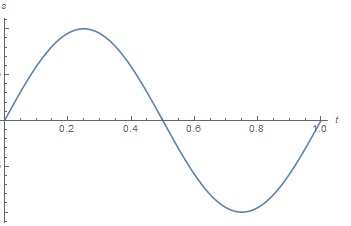
\includegraphics[width=0.6\textwidth]{pig4.jpg}
  \label{Fig1}
\end{figure}


\textbf{\emАЧХ} - амплитудно-частотная характеристика \newline
\textbf{\emФЧХ} - фазочастотная характеристика \newline
\textbf{\emАФЧХ} - амплитудно-фазочастотная характеристика

\par\textbf Из $A$ и $\phi$ можно получить одно комплексное значение \newline
\begin{figure}[H]
 \centering
  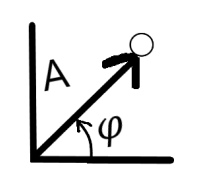
\includegraphics[width=0.2\textwidth]{pig3.jpg}
  \label{Fig2}
\end{figure}
$$A \cos{(2 \pi w t +\phi)}$$ 
$$C \cos{(2 \pi w t)} + S \sin{(2 \pi w t)}$$
$$A (e^{2 \pi i w t} + e^{-2 \pi i w t})/2$$

\par Вспоминая, что $\forall$ непрерывную фунуцию можно разложить в ряд Фурье, получаем:
$$ S(t) = a_{0}/{2} + \sum_{1}^{\infty} (a_{n} \cos{n t} + b_n \sin{n t})$$
\par {\emЧем это плохо?} \newline
Тем, что в качестве частот берутся целые числа $w = 1,2, ... , n$. А у нас и не только целые числа могут встречаться.  \newline
$5 \cos{t} + \cos{2 \pi t}$ и получаем, что $w = 1/(2 \pi) \approx 0.16$  \newline
$$S(t) = \sum_{- \infty}^{\infty} c_{n} e^{i n t}$$  \newline
Найти $c_{n}$ легко, если он нормальный, в нашем случае он нормальный так как разные $e \perp$  \newline
$$ \Rightarrow c_{n} = \int_{- \infty}^{\infty} S(t) e^{i n t} * dt = \int_{- \infty}^{\infty} S(t) e^{-i n t} dt \to \{c_n\}_n^\infty$$
Печально то, что $(c_{5},c_{-5})$ характеризуют одну и ту же частоту 5
$$c_{n} = \int S(t) e^{i w t} dt$$
$$c_{n} \to S^* (w) = \int_{-\infty}^{\infty} s(t) e^{-2 pi i w t} dt$$
$S(t) \to S^* (w) \in \mathbb {C}$ что можно записать в виде $A e^{i \phi}$
\begin{figure}[H]
 \centering
  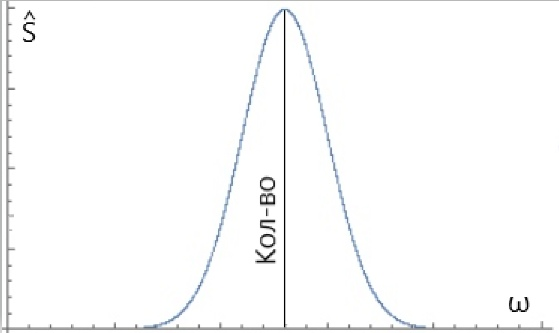
\includegraphics[width=0.6\textwidth]{pig1.jpg}
  \label{Fig3}
\end{figure}

\section{\label{s2}Дельта фунция} \newline
\par 
\par В лабораторной работе был сигнал состоящий из 3 гармоник $S_{L} + S_{M} + S_{H}$, но такой функции не бывает (точнее они плохие, почти везде кроме 3 точек).\newline

\begin{figure}[H]
 \centering
  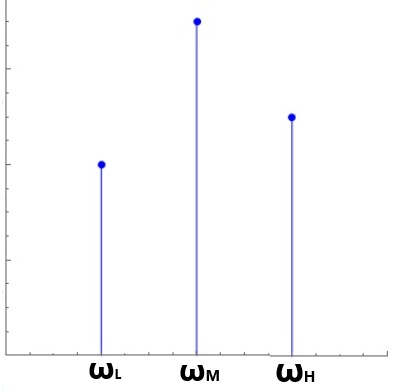
\includegraphics[width=0.6\textwidth]{pig0.jpg}
  \caption{Множество объектов.}
  \label{Fig4}
\end{figure}

\textit{Что же тогда делать?}\newline
Надо придумать обощенную функцию. Пусть $\mathbb {H}$ - множество "хороших" функций.$\mathbb{H} = \{f, g\}$ можно определить скалярное произведение  $\int f(T) g(t) dt$. Если значения будут комплексными, то скалярный квадрат получится отрицательным  \Rightarrow что лучше брать эрмитово произведение $\int f(T) \overline{g(t)} dt$. Пусть есть $\phi$, тогда $\int \# \overline{\phi(t)} dt &$, где вместо $\#$  нужно подставить $f(t)$ \newline
\textit{Как это относится к дельта функции?}\newline
Пусть есть $f(t)$ и $g(t)$, а я хочу научится их считать, значит надо определить операции $f(t)*g(t) \to \mathbb {R}$, но нам надо $f(t)*g(t) \to \mathbb {H}$, но это плохо. Тогда давайте придумаем умнажение, которое будет лучше. На помощь нам придет свертка.
$$f(t) \star g(t) = \int f(t) g(t-\tau) d\tau$$
Нам безразницы какую функцию сдвигать так как получится одно и тоже.\newline
\textit{Есть ли функция, которая может свернуть функцию с ней?}\newline
Да, такой функцией является дельта фунция
\begin{equation*}
\delta(t) = 
 \begin{cases}
   \infty &$t = 0$\\
   0 &$t\neq 0$
 \end{cases}
\end{equation*}
$\int \delta(t) dt = 0$ так как везде 0, кроме одной точки \Rightarrow что верхняя часть должна перевесить. \newline
Обобщенная функция везде 0, кроме $t=0$, а при $t=0$ не определена.
$$\int \delta (t) dt = 1$$
$$\int_{-\infty}^{\infty} f(t) \delta(\tau) dt = f(0)$$
так как она не определена в 0, то
$$\int_{-\epsilon }^{\epsilon} f(t) \delta(t) dt$$ при $\epsilon \to 0 $ получим $f(0)$\newline
\em{Дельта функция из фенкций выбивает ее значение в 0}\newline
\textit{Как найти значение в точке $a$?}
Надо ее перевернуть $f(a) = \int f(t) \delta(t-a)$
\section{\label{s3}Преобразование Фурье}
\par $S(t) \to S^*(w) = \int_{-\infty}^{\infty}S(t) e^{-2 \pi i w t} dt$ \newline
\par 
{\emСвойства}
\begin{enumerate}
	\item линейность
    \item сохраняет форму  $||S*(t) || = ||S(t)||$
    \item $S(t-a) \to e^{-2 \pi i a} S^{*}(w)$
    \item $S(a t) = S^*(w/a)/ |a|$
    \item $S_{1}(t)S_{2}(t) \to S_{1}^*(w) \star S_{2}^*(w)$
    \item $S_{1}(t) \star S_{2}(t) \to S_{1}^*(w) S_{2}^*(w)$
    \item $\overline{S(t)} \to S^*(-w)$
\end{enumerate}       
\par Пусть $S(t) \to S^*(w)$. Надо прнобразовать сигнал в гармоники, но трудность заключается в том, что наш сигнал аналоговый и компьютер его кушать не горит желанием. Надо изучить $S(t)$, а дано $\{S_n\}$. Сигнал бесконечен, а мы имеем только какие-то кго точки и то на определенном отрезке \Rightarrow что у него конечный носитель.

\begin{figure}[H]
 \centering
  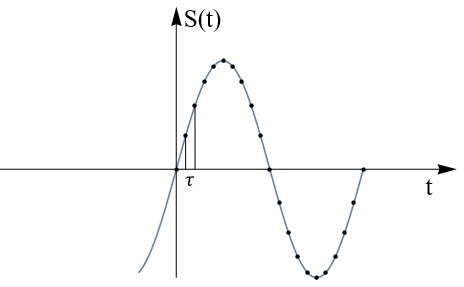
\includegraphics[width=0.6\textwidth]{pig2.jpg}
  \label{Fig5}
\end{figure}

\par \textit{Как законно это исправить?(а точнее бесконечный сигнал запихнуть в коробку)} Нужно воспользоваться $\Sinc{x} = \sin{x}/x$
\par \textit{Как получить точки?} 
\par Гребенка Дирака $\delta(t-1)+\delta(t-2)+...$
$$DiraceComb(t)=\sum_{-\infty}^{\infty} \delta(t-n)$$
$$S(t) \Pi(t) \amalg(t) \to T \tau S^*(w) \star \sinc{T w) \star \amalg(T w)$$
\end{document}